\documentclass[12pt]{article}

%% ── Pacotes ──────────────────────────────────────────────────────────────────
\usepackage[brazil]{babel}
\usepackage[utf8]{inputenc}
\usepackage[T1]{fontenc}
\usepackage{geometry}
\usepackage{amsmath}
\usepackage{graphicx}
\usepackage{caption}
\usepackage{float}
\usepackage[export]{adjustbox}
\usepackage{fancyhdr}
\usepackage{indentfirst}
\usepackage{multicol}        % duas colunas após sumário
\usepackage{booktabs}        % tabelas bonitas
\usepackage{array}
\usepackage{cite}            % citações numéricas ABNT-like
\usepackage{url}
\usepackage{setspace}        % espaçamento
\usepackage{titlesec}        % ajuste de seções
\usepackage{parskip}

%% ── Geometria ABNT ───────────────────────────────────────────────────────────
\geometry{
  a4paper,
  top=3cm, bottom=2cm,
  left=3cm, right=2cm,
  headheight=15pt
}

%% ── Cabeçalho ────────────────────────────────────────────────────────────────
\pagestyle{fancy}
\fancyhf{}
\rhead{\thepage}
\renewcommand{\headrulewidth}{0pt}

%% ── Fonte de figura ──────────────────────────────────────────────────────────
\newcommand{\fonte}[1]{\caption*{\footnotesize Fonte: #1}}

%% ── Espaçamento entre colunas ────────────────────────────────────────────────
\setlength{\columnsep}{0.7cm}
\setlength{\columnseprule}{0pt}

%% ── Tamanho de seção em duas colunas ─────────────────────────────────────────
\titleformat{\section}{\normalfont\large\bfseries}{\thesection}{1em}{}
\titleformat{\subsection}{\normalfont\normalsize\bfseries}{\thesubsection}{1em}{}

%% ═══════════════════════════════════════════════════════════════════════════
\begin{document}

%% ── Capa ─────────────────────────────────────────────────────────────────────
\begin{titlepage}
  \centering
  {\large\textbf{Universidade Federal de Minas Gerais}}\\[0.3cm]
  {\large Engenharia Elétrica}\\[4cm]

  {\large Caio Oliveira Carneiro | Matrícula: 2023059962 \\[0.2cm]
          Diego Felipe Machado Silva | Matrícula: [Inserir Matrícula]\\[0.2cm]
          Guilherme Martins Dijan Domênico | Matrícula: 2022087989\\[0.2cm]
          Ricardo Augusto Costa Brito Moraes | Matrícula: 2022080925}\\[4cm]

  {\Large\textbf{Utilização do Chumbo em Materiais, Componentes e\\[0.2cm]
  Equipamentos Elétricos e Eletrônicos}}\\[4cm]

  \vfill
  {\large Belo Horizonte}\\[0.2cm]
  {\large Maio de 2026}
\end{titlepage}

%% ── Sumário ──────────────────────────────────────────────────────────────────
\newpage
\thispagestyle{empty}
\tableofcontents
\newpage

%% ═══════════════════════════════════════════════════════════════════════════
%% Corpo do trabalho em DUAS COLUNAS
%% ═══════════════════════════════════════════════════════════════════════════
\begin{multicols}{2}
\setstretch{1.0}   % espaçamento simples dentro das colunas

% ─────────────────────────────────────────────────────────────────────────────
\section{Introdução}
% ─────────────────────────────────────────────────────────────────────────────

O chumbo (Pb, número atômico 82) ocupa uma posição historicamente singular na
engenharia elétrica. Sua maleabilidade, baixo ponto de fusão e resistência à corrosão
tornaram-no essencial em duas aplicações críticas: as \textbf{ligas de soldagem} para
interconexões microeletrônicas e os \textbf{sistemas de armazenamento de energia} em
baterias chumbo-ácido \cite{ref_umbrex}.

Ao mesmo tempo, a toxicidade biológica do Pb motivou a Diretiva Europeia de Restrição
de Substâncias Perigosas (RoHS, 2006), que limitou sua concentração em soldas a
\textbf{0,1\% em peso} e forçou uma transição global para ligas \textit{lead-free}
\cite{ref_solder_wiki}. Essa transição, porém, trouxe novos modos de falha, como os
\textit{tin whiskers}, tensionando o compromisso entre desempenho e regulação ambiental
\cite{ref_nasa_whisker}.

Este trabalho aborda o Pb sob quatro eixos: (i)~propriedades físicas, (ii)~processos de
manufatura, (iii)~aspectos microscópicos e (iv)~características de desempenho, com foco
em soldas, baterias e revestimentos de cabos.

% ─────────────────────────────────────────────────────────────────────────────
\section{Propriedades do Chumbo}
% ─────────────────────────────────────────────────────────────────────────────

Localizado no grupo 14, período 6 da tabela periódica, o Pb possui configuração
eletrônica \([Xe]\,4f^{14}\,5d^{10}\,6s^{2}\,6p^{2}\), estados de oxidação predominantes
\(+2\) e \(+4\), e forma rapidamente uma película protetora de óxido/carbonato que cessa
a corrosão subsequente \cite{ref_lead_wiki}.

A Tabela~\ref{tab:propriedades} compara as principais propriedades do Pb puro com o
Sn puro — seu principal parceiro de liga na eletrônica.

% ── ESPAÇO PARA TABELA ───────────────────────────────────────────────────────
\begin{table}[H]
\centering
\caption{Propriedades físicas do Pb e do Sn puros a 20\,°C}
\label{tab:propriedades}
\footnotesize
\begin{tabular}{lcc}
\toprule
\textbf{Propriedade} & \textbf{Pb} & \textbf{Sn} \\
\midrule
Ponto de fusão (°C)               & 327,5  & 231,9  \\
Resistividade ($10^{-7}$\,\(\Omega\)·m) & 2,10   & 1,15   \\
Densidade (g/cm³)                 & 11,35  & 7,30   \\
CTE ($\mu$m/m·K)                  & \(\sim\)29 & \(\sim\)22 \\
Cond. térmica (W/m·K)             & 35,3   & 66,8   \\
Módulo de Young (GPa)             & \(\sim\)16 & \(\sim\)50 \\
\bottomrule
\end{tabular}
\end{table}

O Módulo de Young muito baixo confere ao Pb maleabilidade ímpar: ele absorve
plasticamente tensões mecânicas sem propagar trincas \cite{ref_intel_pkg}. Essa
característica, combinada com o comportamento eutético com o Sn, está na base de suas
aplicações em soldagem.

% ─────────────────────────────────────────────────────────────────────────────
\section{Aplicações na Engenharia Elétrica}
% ─────────────────────────────────────────────────────────────────────────────

\subsection{Liga de Solda Sn-Pb}

A liga eutética \textbf{Sn63Pb37} (63\,\% Sn, 37\,\% Pb em peso) possui ponto de fusão
único em \textbf{183\,°C}, consideravelmente abaixo dos valores dos metais puros
\cite{ref_solder_wiki}. Esse ponto eutético garante solidificação instantânea — sem fase
pastosa — eliminando microfissuras na junta durante o resfriamento \cite{ref_aimsolder}.

A Figura~\ref{fig:diagrama_fase} deve apresentar o diagrama de fase binário Sn-Pb,
destacando o ponto eutético.

% ── ESPAÇO PARA FIGURA ───────────────────────────────────────────────────────
\begin{figure}[H]
  \centering
  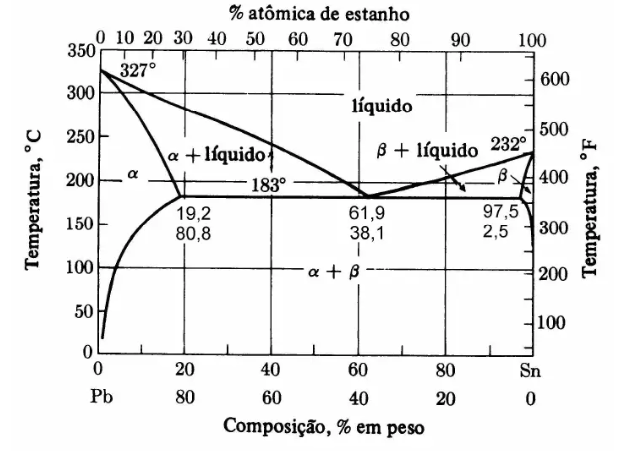
\includegraphics[width=\linewidth]{diagrama_fase_snpb.png}
  \caption{Diagrama de fase binário Sn--Pb.}
  \label{fig:diagrama_fase}
\end{figure}

\subsection{Baterias Chumbo-Ácido}

A reação eletroquímica global da bateria é:

\begin{equation}
  \text{Pb} + \text{PbO}_2 + 2\,\text{H}_2\text{SO}_4
  \;\rightleftharpoons\;
  2\,\text{PbSO}_4 + 2\,\text{H}_2\text{O}
  \label{eq:bateria}
\end{equation}

Durante a descarga (esquerda para direita na Eq.~\ref{eq:bateria}), o anodo de Pb e o
catodo de PbO\(_2\) são convertidos em PbSO\(_4\). O processo é reversível na recarga.
A tecnologia domina \(\approx 70\,\%\) do mercado global de armazenamento estacionário
\cite{ref_bci_circular}.

\subsection{Bainhas de Cabos e Outros Usos}

Em cabos subterrâneos e submarinos de alta tensão (HV/EHV), o Pb extrusado forma
uma barreira impermeável ao vapor d'água, resistente à corrosão microbiológica e aos
hidrocarbonetos do solo — aplicação que polímeros alternativos ainda não substituem com
igual eficácia \cite{ref_epri_pilc}. O Pb também aparece em capacitores piezoelétricos de
titanato-zirconato de chumbo (PZT).

% ─────────────────────────────────────────────────────────────────────────────
\section{Processos de Manufatura}
% ─────────────────────────────────────────────────────────────────────────────

\subsection{Soldagem SMT (Refluxo)}

Na montagem em superfície, a pasta de solda Sn-Pb é depositada por impressão de
estêncil sobre os \textit{pads} da PCB; os componentes são posicionados; e o conjunto
atravessa um forno de refluxo com quatro zonas térmicas controladas:

\begin{enumerate}\itemsep0pt
  \item \textbf{Pré-aquecimento}: rampa de 1--3\,°C/s até $\approx$150\,°C
  \item \textbf{\textit{Soak}}: estabilização por 60--90\,s
  \item \textbf{Refluxo}: pico em $\approx$210\,°C (30\,°C acima do liquidus)
  \item \textbf{Resfriamento}: descida controlada $<$4\,°C/s
\end{enumerate}

A Figura~\ref{fig:perfil_refluxo} ilustra o perfil de temperatura ao longo do forno.

% ── ESPAÇO PARA FIGURA ───────────────────────────────────────────────────────
\begin{figure}[H]
  \centering
  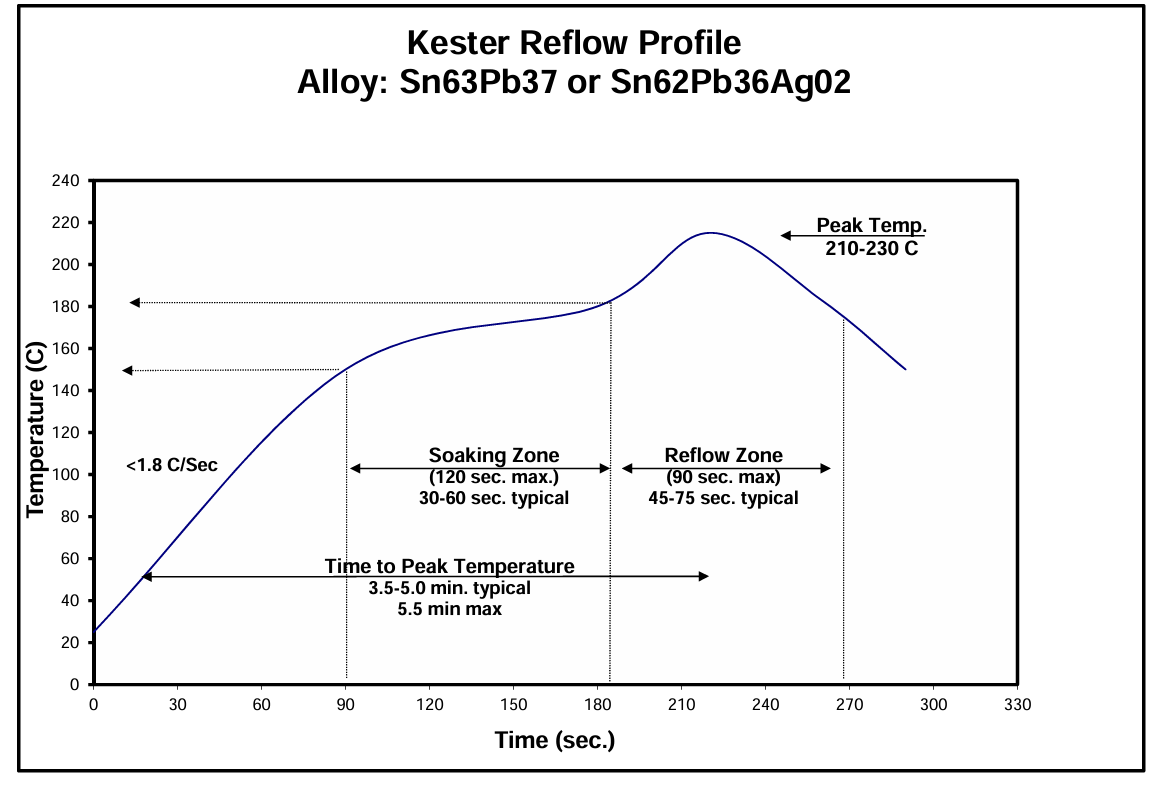
\includegraphics[width=\linewidth]{perfil_refluxo.png}
  \caption{Perfil de temperatura típico de forno de refluxo para Sn63Pb37.}
  \label{fig:perfil_refluxo}
  
\end{figure}

\subsection{Fabricação de Baterias}

O processo de placas chumbo-ácido envolve: (i)~\textbf{fundição das grades} de liga
Pb-Ca ou Pb-Sb; (ii)~\textbf{empastamento} com pasta de PbO + H\(_2\)SO\(_4\) +
aditivos; (iii)~\textbf{cura} em câmara úmida (\(\sim\)50--60\,°C, 48\,h); e
(iv)~\textbf{formação eletroquímica} — primeira carga que converte PbO em Pb (anodo) e
PbO\(_2\) (catodo) \cite{ref_umbrex}.

\subsection{Extrusão de Bainhas de Cabo}

O chumbo (ligado com Sn/Sb para endurecimento) é extrusado continuamente sobre o
núcleo dielétrico do cabo em prensa hidráulica a $\approx$300\,°C, formando uma bainha
tubular de 1--3\,mm de espessura com 100\,\% de estanqueidade radial \cite{ref_epri_pilc}.

\subsection{PZT}

Capacitores piezoelétricos PZT [Pb(Zr,Ti)O\(_3\)] são produzidos por rota cerâmica:
mistura de óxidos → calcinação ($\approx$800\,°C) → sinterização ($\approx$1200\,°C) →
polarização elétrica com campo de $\sim$2\,kV/mm.

% ─────────────────────────────────────────────────────────────────────────────
\section{Aspectos Microscópicos}
% ─────────────────────────────────────────────────────────────────────────────

\subsection{Microestrutura da Solda Sn-Pb}

Na composição eutética, a solidificação gera uma microestrutura bifásica com
\textbf{lamelas alternadas de Sn e Pb} de escala micrométrica (ver Figura~\ref{fig:micro_snpb}).
Essa estrutura fina distribui tensões termomecânicas de forma homogênea, retardando a
nucleação e propagação de microtrincas por fadiga \cite{ref_p2infohouse}.

% ── ESPAÇO PARA FIGURA ───────────────────────────────────────────────────────
\begin{figure}[H]
  \centering
    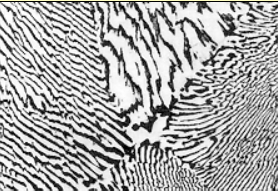
\includegraphics[width=\linewidth]{microestrutura_snpb.png}
    \caption{Microestrutura eutética da liga Sn63Pb37.}
  \label{fig:micro_snpb}
\end{figure}

A presença intergranular de Pb — que \textbf{não forma compostos intermetálicos} com
o Cu nas temperaturas de refluxo SMT — retarda a difusão do Sn livre em direção ao
substrato de cobre, desacelerando o crescimento da camada intermetálica Cu\(_6\)Sn\(_5\)
e CuSn ao longo do envelhecimento térmico \cite{ref_gea_properties}.

\subsection{\textit{Tin Whiskers}}

Nas ligas \textit{lead-free} com alto teor de Sn puro, tensões compressivas residuais na
camada galvânica disparam o crescimento de filamentos monocristalinos de Sn —
os \textit{tin whiskers}. Esses filamentos podem alcançar mais de \textbf{20\,mm} de
comprimento e criar curto-circuitos entre pinos adjacentes \cite{ref_nasa_whisker}. A adição
de apenas \textbf{3--5\,\% de Pb} em peso suprime completamente o fenômeno, pois os
átomos de Pb se inserem nos contornos de grão e eliminam a força motriz compressiva
para a extrusão filamentar \cite{ref_nasa_whisker}.

\subsection{Baterias: Estrutura Porosa e Sulfatação}

As placas de PbO\(_2\) possuem estrutura \textbf{altamente porosa} (porosidade
$\approx$50\,\%), maximizando a área superficial eletroquímica ativa. Em descargas
profundas repetidas, o PbSO\(_4\) gerado recristaliza em grãos grandes e insolúveis —
fenômeno de \textbf{sulfatação} — que obstrui os poros e reduz irreversivelmente a
capacidade da célula \cite{ref_umbrex}.

\subsection{PZT: Estrutura Perovskita}

O PZT apresenta estrutura \textbf{perovskita} ABO\(_3\), onde o Pb\(^{2+}\) ocupa o
sítio A. Abaixo da temperatura de Curie, o deslocamento assimétrico do cátion B
(Zr\(^{4+}\)/Ti\(^{4+}\)) gera polarização espontânea e domínios ferroelétricos, base do
efeito piezoelétrico. A Figura~\ref{fig:perovskita} deve mostrar a célula unitária com o
deslocamento iônico.

% ── ESPAÇO PARA FIGURA ───────────────────────────────────────────────────────
\begin{figure}[H]
  \centering
  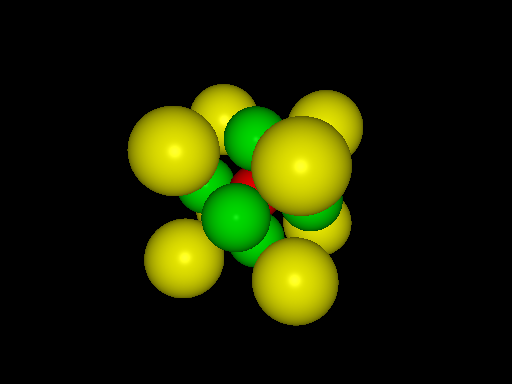
\includegraphics[width=\linewidth]{perovskita_pzt.png}
  \caption{Estrutura perovskita do PZT com polarização espontânea.}
  \label{fig:perovskita}
 
\end{figure}

% ─────────────────────────────────────────────────────────────────────────────
\section{Desempenho e Comparativo}
% ─────────────────────────────────────────────────────────────────────────────

\subsection{Solda: Sn63Pb37 vs.\ SAC (\textit{Lead-Free})}

Embora as ligas SAC (ex.: SAC305 — Sn96,5/Ag3,0/Cu0,5) apresentem maior resistência
à tração (UTS $\approx$5,73\,ksi vs.\ 4,92\,ksi) e dureza Rockwell superior (13,5 vs.\ 10,1),
seu \textbf{Módulo de Young mais elevado} (7,42\,msi vs.\ 4,87\,msi) implica transmissão
direta de tensões termomecânicas ao componente e ao laminado, acelerando a fadiga
\cite{ref_p2infohouse}. A Tabela~\ref{tab:soldas} consolida o comparativo.

\begin{table}[H]
\centering
\caption{Propriedades mecânicas: Sn63Pb37 vs.\ SAC}
\label{tab:soldas}
\footnotesize
\begin{tabular}{lcc}
\toprule
\textbf{Propriedade}         & \textbf{Sn63Pb37} & \textbf{SAC} \\
\midrule
UTS (ksi)                    & 4,92              & 5,73         \\
Escoamento (ksi)             & 4,38              & 4,86         \\
Young (msi)                  & 4,87              & 7,42         \\
Dureza (Rockwell 15W)        & 10,1              & 13,5         \\
Cond.\ térmica (W/m·K)      & 50,0              & 57,3         \\
Fusão (°C)                   & 183 (exato)       & 215--217     \\
\bottomrule
\end{tabular}
\end{table}

Adicionalmente, ligas com traços de apenas \textbf{0,5\,\% de Pb} contaminando uma
SAC reduziram a vida em fadiga de $\approx$13.400 ciclos para $\approx$6.320 ciclos —
queda de $\sim$53\,\% — evidenciando a incompatibilidade microestrutural de misturas
não eutéticas \cite{ref_p2infohouse}.

\subsection{Baterias: Chumbo-Ácido vs.\ Íon-Lítio}

A Tabela~\ref{tab:baterias} apresenta comparativo entre as duas tecnologias para
aplicações estacionárias (UPS de subestação).

\begin{table}[H]
\centering
\caption{Comparativo chumbo-ácido vs.\ íon-lítio (uso estacionário)}
\label{tab:baterias}
\resizebox{\linewidth}{!}{%  <--- COMANDO ADICIONADO AQUI
\begin{tabular}{lcc}
\toprule
\textbf{Critério}           & \textbf{Pb-ácido} & \textbf{Li-íon}  \\
\midrule
Densidade de energia (Wh/kg) & 30--50           & 100--250         \\
Ciclo de vida (ciclos)       & 200--500         & 500--2000        \\
Taxa de reciclagem (\%)      & $\approx$99      & $\approx$15      \\
Risco \textit{thermal runaway} & Não            & Sim              \\
Necessidade de BMS           & Não              & Sim              \\
Custo relativo (R\$/kWh)    & Baixo            & Alto             \\
\bottomrule
\end{tabular}%
} % <--- FECHAMENTO DO COMANDO AQUI
\end{table}

A bateria chumbo-ácido domina $\approx$76\,\% do parque de UPS de subestações
brasileiras e mundiais, principalmente por sua \textbf{capacidade de corrente de surto},
operação passiva sem BMS e histórico secular de confiabilidade \cite{ref_sandia,ref_swiftpower}.

\subsection{Regulação: RoHS e Isenções}

A Diretiva RoHS restringe o Pb a 0,1\,\% em equipamentos de consumo, mas mantém
isenções para aplicações aeroespaciais, militares e médicas. A NASA e a ESA proíbem
revestimentos de Sn puro em seus circuitos devido ao risco de \textit{tin whiskers} —
utilizando exclusivamente Sn-Pb certificado \cite{ref_nasa_whisker}.

O gráfico da Figura~\ref{fig:ciclos_fadiga} deve comparar a vida em fadiga (ciclos) de
juntas Sn-Pb vs.\ SAC sob ciclagem térmica $-40$\,°C a $+125$\,°C.

% ── ESPAÇO PARA FIGURA ───────────────────────────────────────────────────────
\begin{figure}[H]
  \centering
  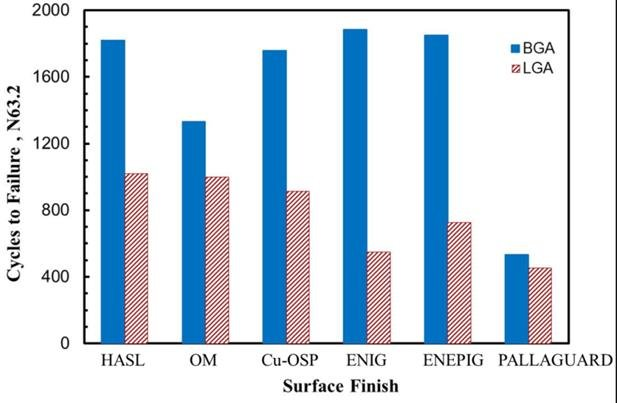
\includegraphics[width=\linewidth]{fadiga_snpb_sac.png}
  \caption{Comparativo de confiabilidade em fadiga térmica.}
  \label{fig:ciclos_fadiga}
\end{figure}

% ─────────────────────────────────────────────────────────────────────────────
\section{Conclusão}
% ─────────────────────────────────────────────────────────────────────────────

O chumbo permanece insubstituível em três nichos críticos da engenharia elétrica: nas
ligas de solda de alta confiabilidade (sistemas aeroespaciais e médicos), nas baterias
chumbo-ácido estacionárias e nos revestimentos de cabos subterrâneos/submarinos. Suas
propriedades microscópicas — maleabilidade eutética, supressão de \textit{tin whiskers} e
impermeabilidade passiva — ainda não encontram equivalentes técnicos de igual custo e
maturidade industrial.

O desafio da engenharia moderna é administrar o \textbf{paradoxo Pb}: restringir seu uso
nos produtos de consumo descartáveis (onde a regulação ambiental é plenamente
justificada) enquanto preserva, com rastreabilidade e reciclagem em circuito fechado de
99\,\%, sua presença nos sistemas de missão crítica onde a falha tem consequências
catastróficas. A transição tecnológica depende de avanços na compreensão dos mecanismos
de \textit{whisker} e no desenvolvimento de ligas \textit{lead-free} com complacência
mecânica equivalente à da Sn63Pb37.

\end{multicols}

%% ── Referências ──────────────────────────────────────────────────────────────
\newpage
\begin{thebibliography}{99}
\small

\bibitem{ref_umbrex}
UMBREX. \textit{Lead Acid Batteries}. Disponível em:
\url{https://umbrex.com/resources/energy-industry-glossary/energy-storage-glossary/lead-acid-batteries/}.
Acesso em: 26 maio 2026.

\bibitem{ref_solder_wiki}
WIKIPEDIA. \textit{Solder}. Disponível em: \url{https://en.wikipedia.org/wiki/Solder}.
Acesso em: 26 maio 2026.

\bibitem{ref_nasa_whisker}
BARR, T. \textit{Mitigating and Preventing the Growth of Tin and Other Metal Whiskers on
Critical Hardware}. NASA NEPP, 2007. Disponível em:
\url{https://nepp.nasa.gov/whisker/reference/tech_papers/2007-barr-paper-mitigating-whiskers.pdf}.
Acesso em: 26 maio 2026.

\bibitem{ref_lead_wiki}
WIKIPEDIA. \textit{Lead}. Disponível em: \url{https://en.wikipedia.org/wiki/Lead}.
Acesso em: 26 maio 2026.

\bibitem{ref_intel_pkg}
INTEL. \textit{Physical Constants of IC Package Materials}. Disponível em:
\url{https://www.intel.com/content/dam/www/public/us/en/documents/packaging-databooks/packaging-chapter-05-databook.pdf}.
Acesso em: 26 maio 2026.

\bibitem{ref_aimsolder}
AIM SOLDER. \textit{Choosing a Solder Alloy: What You Need to Know}. Disponível em:
\url{https://www.aimsolder.com/blog/choosing-a-solder-alloy-what-you-need-to-know/}.
Acesso em: 26 maio 2026.

\bibitem{ref_bci_circular}
BATTERY COUNCIL INTERNATIONAL. \textit{What Role Can Lead-Acid Batteries Play in the
Circular Economy?} Disponível em:
\url{https://batterycouncil.org/news/essential-insights/what-role-can-lead-acid-batteries-play-in-the-circular-economy/}.
Acesso em: 26 maio 2026.

\bibitem{ref_epri_pilc}
EPRI. \textit{Environmental Impacts of Lead from Paper-Insulated Lead-Covered Cables}.
Relatório n.º 1009513. Palo Alto, CA: EPRI, 2005.

\bibitem{ref_p2infohouse}
P2 INFOHOUSE. \textit{Properties and Comparison of Lead-Free Solders}. Disponível em:
\url{https://p2infohouse.org/ref/37/36617.pdf}. Acesso em: 26 maio 2026.

\bibitem{ref_gea_properties}
GLOBAL ELECTRONICS ASSOCIATION. \textit{Properties That are Important in Lead-Free
Solders}. Disponível em:
\url{https://www.electronics.org/system/files/technical_resource/E9%26S18_01.pdf}.
Acesso em: 26 maio 2026.

\bibitem{ref_sandia}
KEY, T. \textit{Assessment of Alternatives to Lead-Acid Substation Batteries}. Sandia
National Laboratories, 2003. Disponível em:
\url{https://www.sandia.gov/ess-ssl/EESAT/2003_papers/Key.pdf}. Acesso em: 26 maio 2026.

\bibitem{ref_swiftpower}
SWIFT POWER. \textit{Understanding Substation Batteries: Types, Functions, and
Importance}. Disponível em:
\url{https://swiftpower.com/understanding-substation-batteries-types-functions-importance/}.
Acesso em: 26 maio 2026.

\bibitem{ref_vertiv}
VERTIV. \textit{Assessment of Alternatives to Lead-Acid Batteries for Substations}.
BattCon 2004. Disponível em:
\url{https://www.vertiv.com/48e16b/globalassets/documents/battcon-static-assets/2004/assessment-of-alternatives-to-lead-acid-batteries-for-substations.pdf}.
Acesso em: 26 maio 2026.

\end{thebibliography}

\end{document}